\section{Objectives}

\begin{frame}{Environmental Influence on the Phenotype}
  \begin{columns}
\begin{column}{0.6\textwidth}
\begin{itemize}
	\item in biology, genotype not sole determinant of phenotype
    \item $P = G + E$
    \item plasticity: phenotypic response to the environment
    \item how does environmental influence on the phenotype affect evolvability?
\end{itemize}
\end{column}
\begin{column}{0.4\textwidth}
\begin{center}
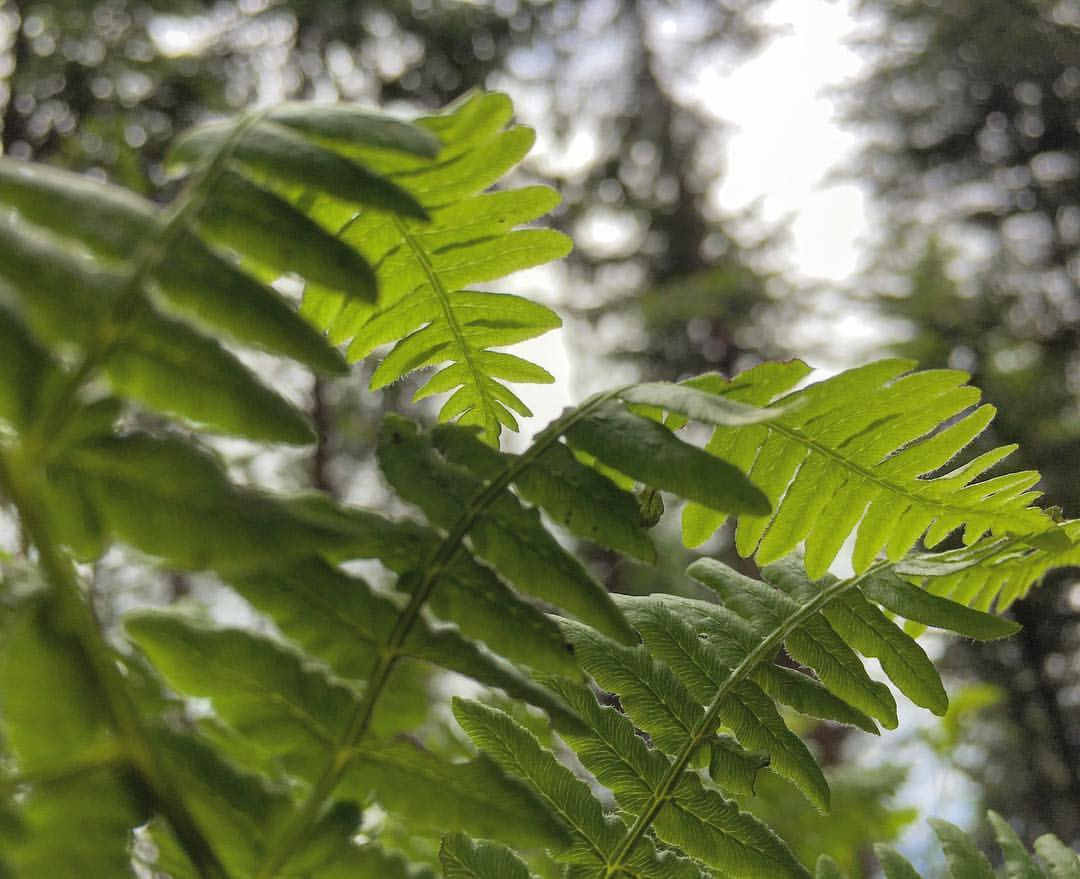
\includegraphics[width=\textwidth,trim={12cm 0 6cm 0},clip]{img/bent_fern}
\end{center}
\end{column}
\end{columns}
\end{frame}

\begin{frame}{Motivation: Practical and Scientific}
\begin{columns}
\begin{column}{0.6\textwidth}
\begin{figure}
  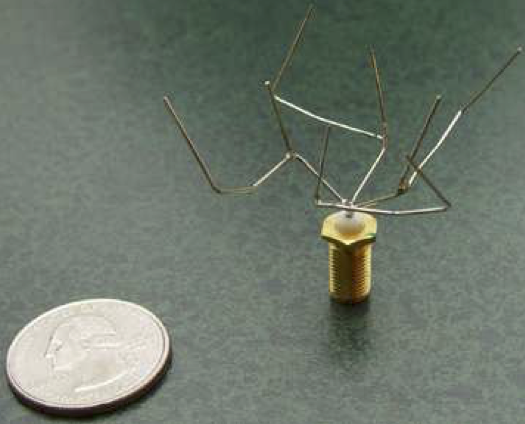
\includegraphics[width=\textwidth]{img/evolved_antenna} 
  \hspace{2ex}
  \caption{A spacecraft antenna design generated using evolutionary methods \cite[Figure 2(a)]{Hornby2006AutomatedAlgorithms}.}
  \label{fig:evolved_antenna}
\end{figure}
\end{column}
\begin{column}{0.4\textwidth}
\begin{center}
\begin{figure}
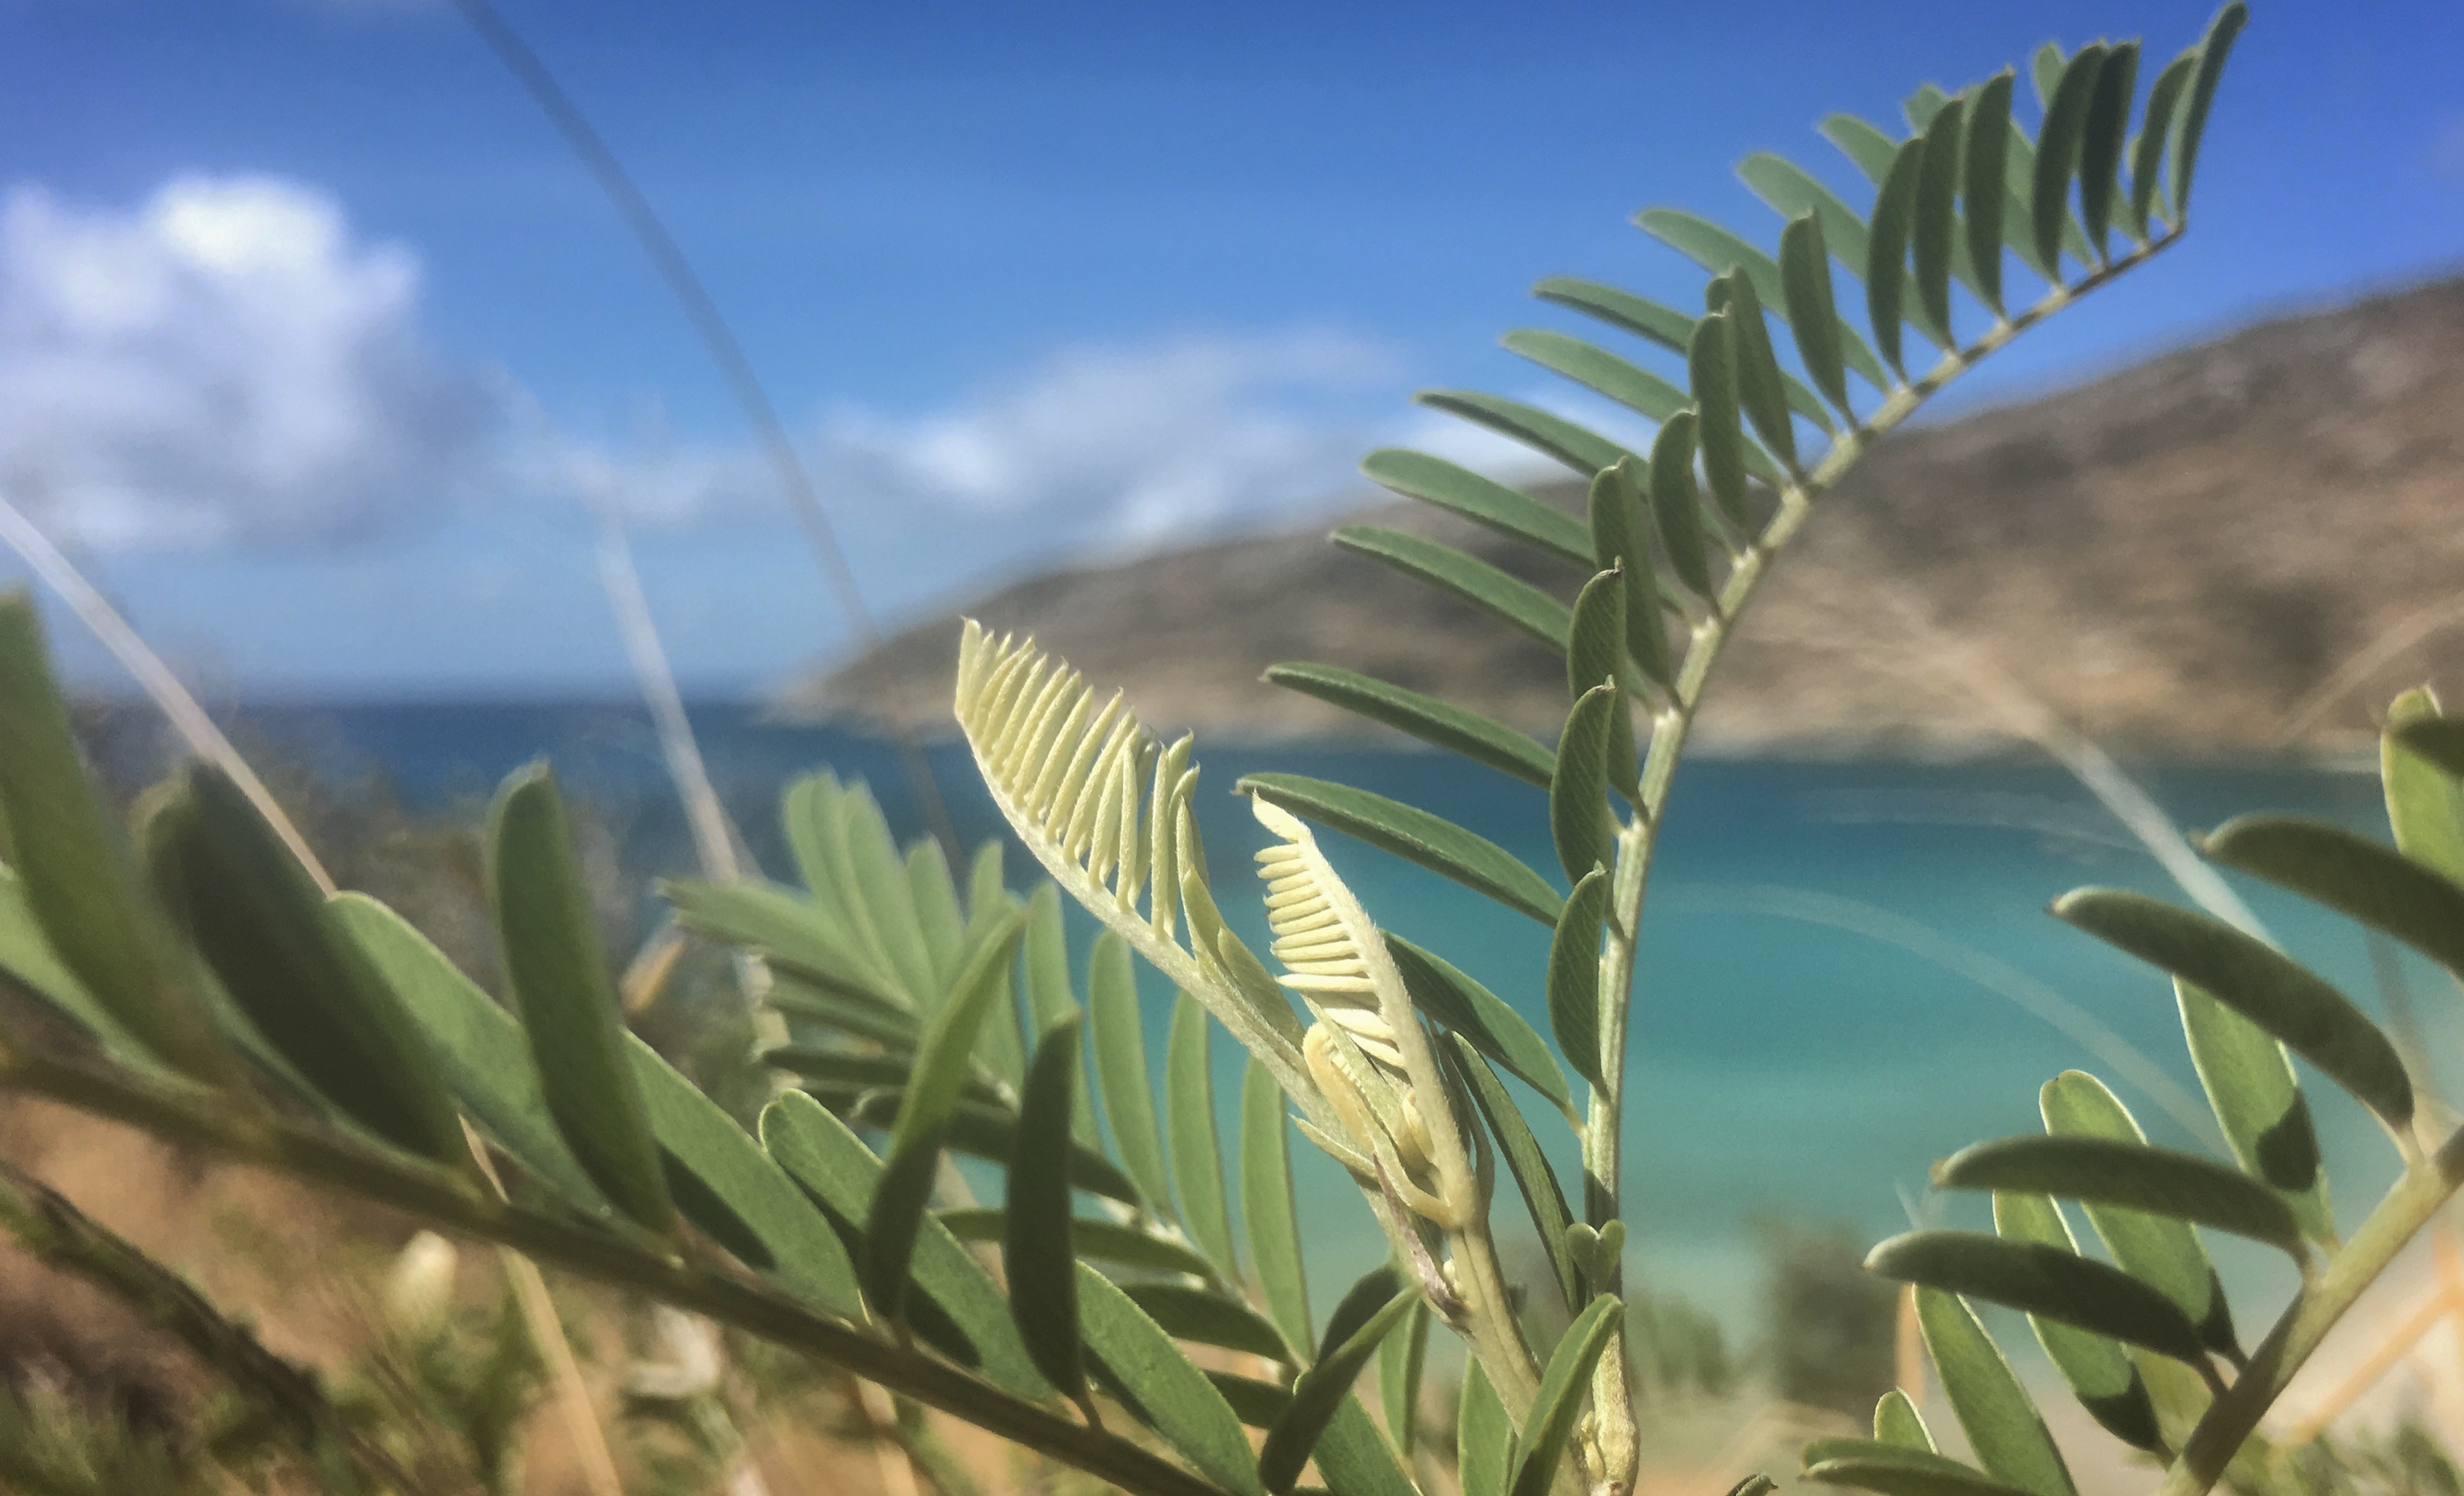
\includegraphics[width=\textwidth,trim={43cm 0 47cm 8cm},clip]{img/island_fern}
\caption{A biological frond design generated via evolution.}
\end{figure}
\end{center}
\end{column}
\end{columns}
\end{frame}